% Standalone — compile with pdflatex or upload to Overleaf
\documentclass[border=8pt]{standalone}
\usepackage[T1]{fontenc}
\usepackage{lmodern}
\usepackage{pgfplots}
\pgfplotsset{compat=1.18}

\begin{document}
  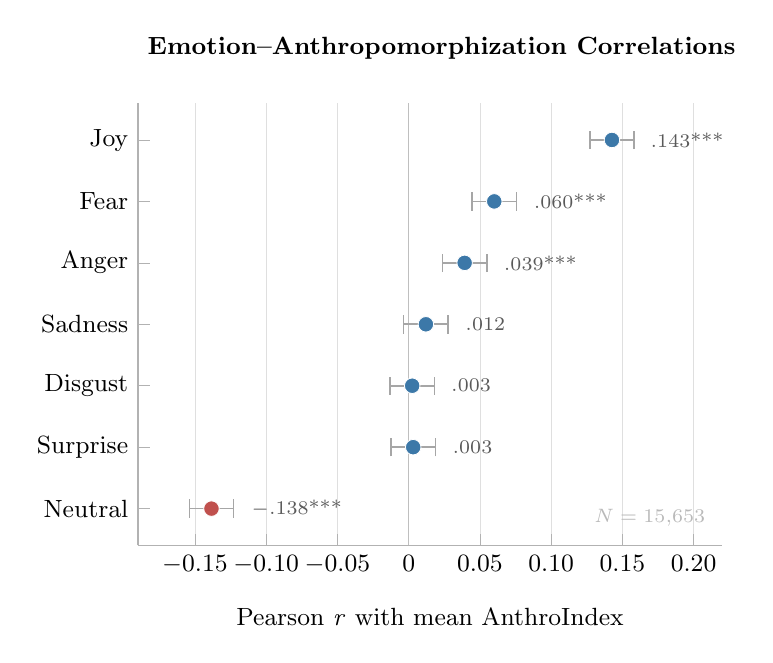
\begin{tikzpicture}
    \begin{axis}[
      width=9cm,
      height=7.2cm,
      clip=false,
      xmin=-0.19, xmax=0.22,
      ymin=-0.6,  ymax=6.6,
      xtick={-0.15,-0.10,-0.05,0,0.05,0.10,0.15,0.20},
      xticklabels={$-$0.15, $-$0.10, $-$0.05, 0, 0.05, 0.10, 0.15, 0.20},
      xticklabel style={font=\small},
      xlabel={Pearson \textit{r} with mean AnthroIndex},
      xlabel style={font=\small, at={(0.5,-0.12)}},
      ytick={0,1,2,3,4,5,6},
      yticklabels={Neutral, Surprise, Disgust, Sadness, Anger, Fear, Joy},
      yticklabel style={font=\small, anchor=east},
      xmajorgrids=true,
      grid style={gray!25, very thin},
      axis x line*=bottom,
      axis y line*=left,
      every outer x axis line/.append style={gray!60},
      every outer y axis line/.append style={gray!60},
      tick style={gray!60},
      title={\textbf{Emotion--Anthropomorphization Correlations}},
      title style={font=\small, at={(0.0,1.04)}, anchor=south west},
    ]

      \draw[gray!50, thin] (0, -0.6) -- (0, 6.6);

      % Joy
      \draw[gray!70, semithick] (0.1272,6)--(0.1582,6);
      \draw[gray!70, semithick] (0.1272,5.85)--(0.1272,6.15);
      \draw[gray!70, semithick] (0.1582,5.85)--(0.1582,6.15);
      % Fear
      \draw[gray!70, semithick] (0.0445,5)--(0.0758,5);
      \draw[gray!70, semithick] (0.0445,4.85)--(0.0445,5.15);
      \draw[gray!70, semithick] (0.0758,4.85)--(0.0758,5.15);
      % Anger
      \draw[gray!70, semithick] (0.0237,4)--(0.0550,4);
      \draw[gray!70, semithick] (0.0237,3.85)--(0.0237,4.15);
      \draw[gray!70, semithick] (0.0550,3.85)--(0.0550,4.15);
      % Sadness
      \draw[gray!70, semithick] (-0.0036,3)--(0.0277,3);
      \draw[gray!70, semithick] (-0.0036,2.85)--(-0.0036,3.15);
      \draw[gray!70, semithick] (0.0277,2.85)--(0.0277,3.15);
      % Disgust
      \draw[gray!70, semithick] (-0.0132,2)--(0.0181,2);
      \draw[gray!70, semithick] (-0.0132,1.85)--(-0.0132,2.15);
      \draw[gray!70, semithick] (0.0181,1.85)--(0.0181,2.15);
      % Surprise
      \draw[gray!70, semithick] (-0.0124,1)--(0.0189,1);
      \draw[gray!70, semithick] (-0.0124,0.85)--(-0.0124,1.15);
      \draw[gray!70, semithick] (0.0189,0.85)--(0.0189,1.15);
      % Neutral
      \draw[gray!70, semithick] (-0.1539,0)--(-0.1229,0);
      \draw[gray!70, semithick] (-0.1539,-0.15)--(-0.1539,0.15);
      \draw[gray!70, semithick] (-0.1229,-0.15)--(-0.1229,0.15);

      % Positive dots
      \addplot[only marks, mark=*, mark size=2.8pt,
               fill={rgb,255:red,60;green,120;blue,168},
               draw=white, line width=0.3pt]
        coordinates {(0.1427,6)(0.0601,5)(0.0393,4)(0.0121,3)(0.0025,2)(0.0032,1)};
      % Negative dot
      \addplot[only marks, mark=*, mark size=2.8pt,
               fill={rgb,255:red,192;green,80;blue,77},
               draw=white, line width=0.3pt]
        coordinates {(-0.1384,0)};

      % Labels — all on the right
      \node[anchor=west, font=\scriptsize, text=gray!70!black] at (0.163,6)  {$.143$\rlap{***}};
      \node[anchor=west, font=\scriptsize, text=gray!70!black] at (0.081,5)  {$.060$\rlap{***}};
      \node[anchor=west, font=\scriptsize, text=gray!70!black] at (0.060,4)  {$.039$\rlap{***}};
      \node[anchor=west, font=\scriptsize, text=gray!70!black] at (0.033,3)  {$.012$};
      \node[anchor=west, font=\scriptsize, text=gray!70!black] at (0.023,2)  {$.003$};
      \node[anchor=west, font=\scriptsize, text=gray!70!black] at (0.024,1)  {$.003$};
      \node[anchor=west, font=\scriptsize, text=gray!70!black] at (-0.117,0) {$-.138$\rlap{***}};

      \node[anchor=south east, font=\scriptsize, text=gray!55]
        at (axis cs:0.215,-0.45) {$N = 15{,}653$};
    \end{axis}
  \end{tikzpicture}
\end{document}
